% Options for packages loaded elsewhere
\PassOptionsToPackage{unicode}{hyperref}
\PassOptionsToPackage{hyphens}{url}
\documentclass[a4paper]{article}
\usepackage[a4paper,margin=22mm]{geometry}
\usepackage{xcolor}
\usepackage{amsmath,amssymb}
\setcounter{secnumdepth}{-\maxdimen} % remove section numbering
\usepackage{iftex}
\ifPDFTeX
  \usepackage[T1]{fontenc}
  \usepackage[utf8]{inputenc}
  \usepackage{textcomp} % provide euro and other symbols
\else % if luatex or xetex
  \usepackage{unicode-math} % this also loads fontspec
  \defaultfontfeatures{Scale=MatchLowercase}
  \defaultfontfeatures[\rmfamily]{Ligatures=TeX,Scale=1}
\fi
\usepackage{lmodern}
\ifPDFTeX\else
  % xetex/luatex font selection
\fi
% Use upquote if available, for straight quotes in verbatim environments
\IfFileExists{upquote.sty}{\usepackage{upquote}}{}
\IfFileExists{microtype.sty}{% use microtype if available
  \usepackage[]{microtype}
  \UseMicrotypeSet[protrusion]{basicmath} % disable protrusion for tt fonts
}{}
\makeatletter
\@ifundefined{KOMAClassName}{% if non-KOMA class
  \IfFileExists{parskip.sty}{%
    \usepackage{parskip}
  }{% else
    \setlength{\parindent}{0pt}
    \setlength{\parskip}{6pt plus 2pt minus 1pt}}
}{% if KOMA class
  \KOMAoptions{parskip=half}}
\makeatother
\usepackage{color}
\usepackage{fancyvrb}
\newcommand{\VerbBar}{|}
\newcommand{\VERB}{\Verb[commandchars=\\\{\}]}
\DefineVerbatimEnvironment{Highlighting}{Verbatim}{commandchars=\\\{\}}
% Add ',fontsize=\small' for more characters per line
\newenvironment{Shaded}{}{}
\newcommand{\AlertTok}[1]{\textcolor[rgb]{1.00,0.00,0.00}{\textbf{#1}}}
\newcommand{\AnnotationTok}[1]{\textcolor[rgb]{0.38,0.63,0.69}{\textbf{\textit{#1}}}}
\newcommand{\AttributeTok}[1]{\textcolor[rgb]{0.49,0.56,0.16}{#1}}
\newcommand{\BaseNTok}[1]{\textcolor[rgb]{0.25,0.63,0.44}{#1}}
\newcommand{\BuiltInTok}[1]{\textcolor[rgb]{0.00,0.50,0.00}{#1}}
\newcommand{\CharTok}[1]{\textcolor[rgb]{0.25,0.44,0.63}{#1}}
\newcommand{\CommentTok}[1]{\textcolor[rgb]{0.38,0.63,0.69}{\textit{#1}}}
\newcommand{\CommentVarTok}[1]{\textcolor[rgb]{0.38,0.63,0.69}{\textbf{\textit{#1}}}}
\newcommand{\ConstantTok}[1]{\textcolor[rgb]{0.53,0.00,0.00}{#1}}
\newcommand{\ControlFlowTok}[1]{\textcolor[rgb]{0.00,0.44,0.13}{\textbf{#1}}}
\newcommand{\DataTypeTok}[1]{\textcolor[rgb]{0.56,0.13,0.00}{#1}}
\newcommand{\DecValTok}[1]{\textcolor[rgb]{0.25,0.63,0.44}{#1}}
\newcommand{\DocumentationTok}[1]{\textcolor[rgb]{0.73,0.13,0.13}{\textit{#1}}}
\newcommand{\ErrorTok}[1]{\textcolor[rgb]{1.00,0.00,0.00}{\textbf{#1}}}
\newcommand{\ExtensionTok}[1]{#1}
\newcommand{\FloatTok}[1]{\textcolor[rgb]{0.25,0.63,0.44}{#1}}
\newcommand{\FunctionTok}[1]{\textcolor[rgb]{0.02,0.16,0.49}{#1}}
\newcommand{\ImportTok}[1]{\textcolor[rgb]{0.00,0.50,0.00}{\textbf{#1}}}
\newcommand{\InformationTok}[1]{\textcolor[rgb]{0.38,0.63,0.69}{\textbf{\textit{#1}}}}
\newcommand{\KeywordTok}[1]{\textcolor[rgb]{0.00,0.44,0.13}{\textbf{#1}}}
\newcommand{\NormalTok}[1]{#1}
\newcommand{\OperatorTok}[1]{\textcolor[rgb]{0.40,0.40,0.40}{#1}}
\newcommand{\OtherTok}[1]{\textcolor[rgb]{0.00,0.44,0.13}{#1}}
\newcommand{\PreprocessorTok}[1]{\textcolor[rgb]{0.74,0.48,0.00}{#1}}
\newcommand{\RegionMarkerTok}[1]{#1}
\newcommand{\SpecialCharTok}[1]{\textcolor[rgb]{0.25,0.44,0.63}{#1}}
\newcommand{\SpecialStringTok}[1]{\textcolor[rgb]{0.73,0.40,0.53}{#1}}
\newcommand{\StringTok}[1]{\textcolor[rgb]{0.25,0.44,0.63}{#1}}
\newcommand{\VariableTok}[1]{\textcolor[rgb]{0.10,0.09,0.49}{#1}}
\newcommand{\VerbatimStringTok}[1]{\textcolor[rgb]{0.25,0.44,0.63}{#1}}
\newcommand{\WarningTok}[1]{\textcolor[rgb]{0.38,0.63,0.69}{\textbf{\textit{#1}}}}
\usepackage{longtable,booktabs,array,tabularx}
\usepackage{tikz}
\usetikzlibrary{arrows.meta,positioning,fit,calc,shapes.geometric,shapes.multipart}
\usepackage{calc} % for calculating minipage widths
% Correct order of tables after \paragraph or \subparagraph
\usepackage{etoolbox}
\makeatletter
\patchcmd\longtable{\par}{\if@noskipsec\mbox{}\fi\par}{}{}
\makeatother
% Allow footnotes in longtable head/foot
\IfFileExists{footnotehyper.sty}{\usepackage{footnotehyper}}{\usepackage{footnote}}
\makesavenoteenv{longtable}
\usepackage{graphicx}
\makeatletter
\newsavebox\pandoc@box
\newcommand*\pandocbounded[1]{% scales image to fit in text height/width
  \sbox\pandoc@box{#1}%
  \Gscale@div\@tempa{\textheight}{\dimexpr\ht\pandoc@box+\dp\pandoc@box\relax}%
  \Gscale@div\@tempb{\linewidth}{\wd\pandoc@box}%
  \ifdim\@tempb\p@<\@tempa\p@\let\@tempa\@tempb\fi% select the smaller of both
  \ifdim\@tempa\p@<\p@\scalebox{\@tempa}{\usebox\pandoc@box}%
  \else\usebox{\pandoc@box}%
  \fi%
}
% Set default figure placement to htbp
\def\fps@figure{htbp}
\makeatother
\setlength{\emergencystretch}{3em} % prevent overfull lines
\setlength{\tabcolsep}{8pt}
\providecommand{\tightlist}{%
  \setlength{\itemsep}{0pt}\setlength{\parskip}{0pt}}
\usepackage{bookmark}
\IfFileExists{xurl.sty}{\usepackage{xurl}}{} % add URL line breaks if available
\urlstyle{same}
\hypersetup{
  pdftitle={AI1220 System Design Document},
  hidelinks,
  pdfcreator={LaTeX via pandoc}}
\newcolumntype{Y}{>{\raggedright\arraybackslash}X}
\newcolumntype{L}[1]{>{\raggedright\arraybackslash}p{#1}}
\newcommand{\diagramlabel}[1]{\textbf{#1}}
\tikzset{
  box/.style={draw=black!55, rounded corners=4pt, fill=black!2, align=center, minimum width=26mm, minimum height=10mm},
  extbox/.style={draw=black!55, rounded corners=4pt, fill=black!7, align=center, minimum width=28mm, minimum height=10mm},
  datastore/.style={draw=black!55, rounded corners=4pt, fill=black!4, align=center, minimum width=24mm, minimum height=10mm},
  line/.style={-{Latex[length=2.2mm]}, draw=black!65, thick},
  noteedge/.style={draw=black!50, thick},
}

\title{AI1220 System Design Document}
\author{}
\date{}

\begin{document}
\maketitle

\section{AI1220 System Design
Document}\label{ai1220-system-design-document}

\subsection{Collaborative Document Editor with AI Writing
Assistant}\label{collaborative-document-editor-with-ai-writing-assistant}

Version: 1.0\\
Scope: AI1220 Assignment, System Architecture Deliverable\\
Repository basis: current implementation in this repository as of April
3, 2026

\subsection{1. Purpose}\label{1-purpose}

This document provides the architecture content required for the AI1220
assignment. It covers:

\begin{itemize}
\tightlist
\item
  architectural drivers
\item
  C4 system context, container, and component views
\item
  feature decomposition
\item
  AI integration design
\item
  API design
\item
  authentication and authorization
\item
  communication model
\item
  code structure and repository organization
\item
  data model
\item
  architecture decision records
\end{itemize}

This version is intentionally aligned to the current repository
implementation, not only to an ideal target architecture. Where the
codebase is still using prototype persistence or local-development
shortcuts, that is stated explicitly.

\subsection{2. Architectural Drivers}\label{2-architectural-drivers}

\begin{table}[h]
\small
\begin{tabularx}{\textwidth}{@{}L{9mm}L{43mm}Y@{}}
\toprule
Rank & Driver & Why it matters \\
\midrule
1 & Reliable realtime collaboration & Concurrent editing is the core product behavior. If sessions do not converge, the product fails. \\
2 & Safe AI assistance during collaboration & AI must produce reviewable proposals rather than silently overwriting newer human edits. \\
3 & Correct permission enforcement & Owner, editor, commenter, and viewer behavior must remain distinct for editing, AI, export, and version restore. \\
4 & Responsive user experience & Editing, reconnect, comments, and AI status need to feel fast enough for continuous use. \\
5 & Realistic student-team implementation & The architecture must remain decomposable and testable in a monorepo without excessive operational overhead. \\
\bottomrule
\end{tabularx}
\end{table}

These drivers lead to the main design choices:

\begin{itemize}
\tightlist
\item
  push-based collaboration via a dedicated realtime service
\item
  AI returns proposals rather than direct document mutations
\item
  business operations use REST, while live editing uses a persistent
  realtime channel
\item
  metadata and collaborative state are separated
\end{itemize}

\subsection{3. C4 Model}\label{3-c4-model}

\subsubsection{3.1 Level 1: System
Context}\label{31-level-1-system-context}

Mermaid source:
\href{/Users/rayan.banerjee/courses/software\%20project/docs/diagrams/ai1220-system-context.mmd}{ai1220-system-context.mmd}

\begin{figure}[h]
\centering
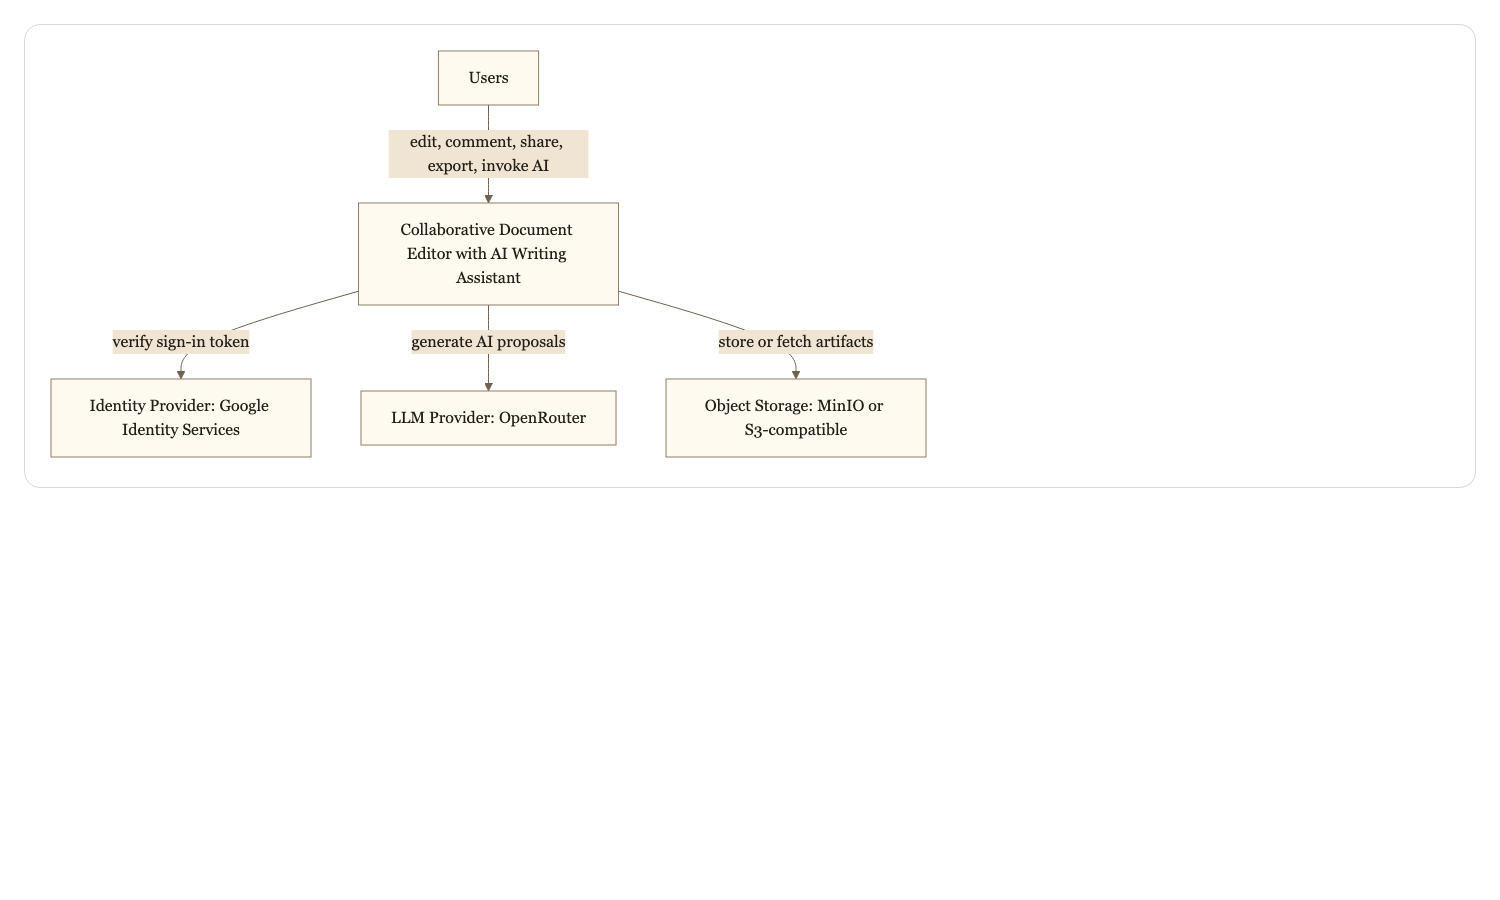
\includegraphics[width=\textwidth,height=0.32\textheight,keepaspectratio]{docs/diagrams/generated/ai1220-system-context.png}
\end{figure}

The system interacts with users, an external identity provider for
sign-in, an LLM provider for AI features, and object storage for export
artifacts and future retained snapshots.

\subsubsection{3.2 Level 2: Container
Diagram}\label{32-level-2-container-diagram}

Mermaid source:
\href{/Users/rayan.banerjee/courses/software\%20project/docs/diagrams/ai1220-container-view.mmd}{ai1220-container-view.mmd}

\begin{figure}[h]
\centering
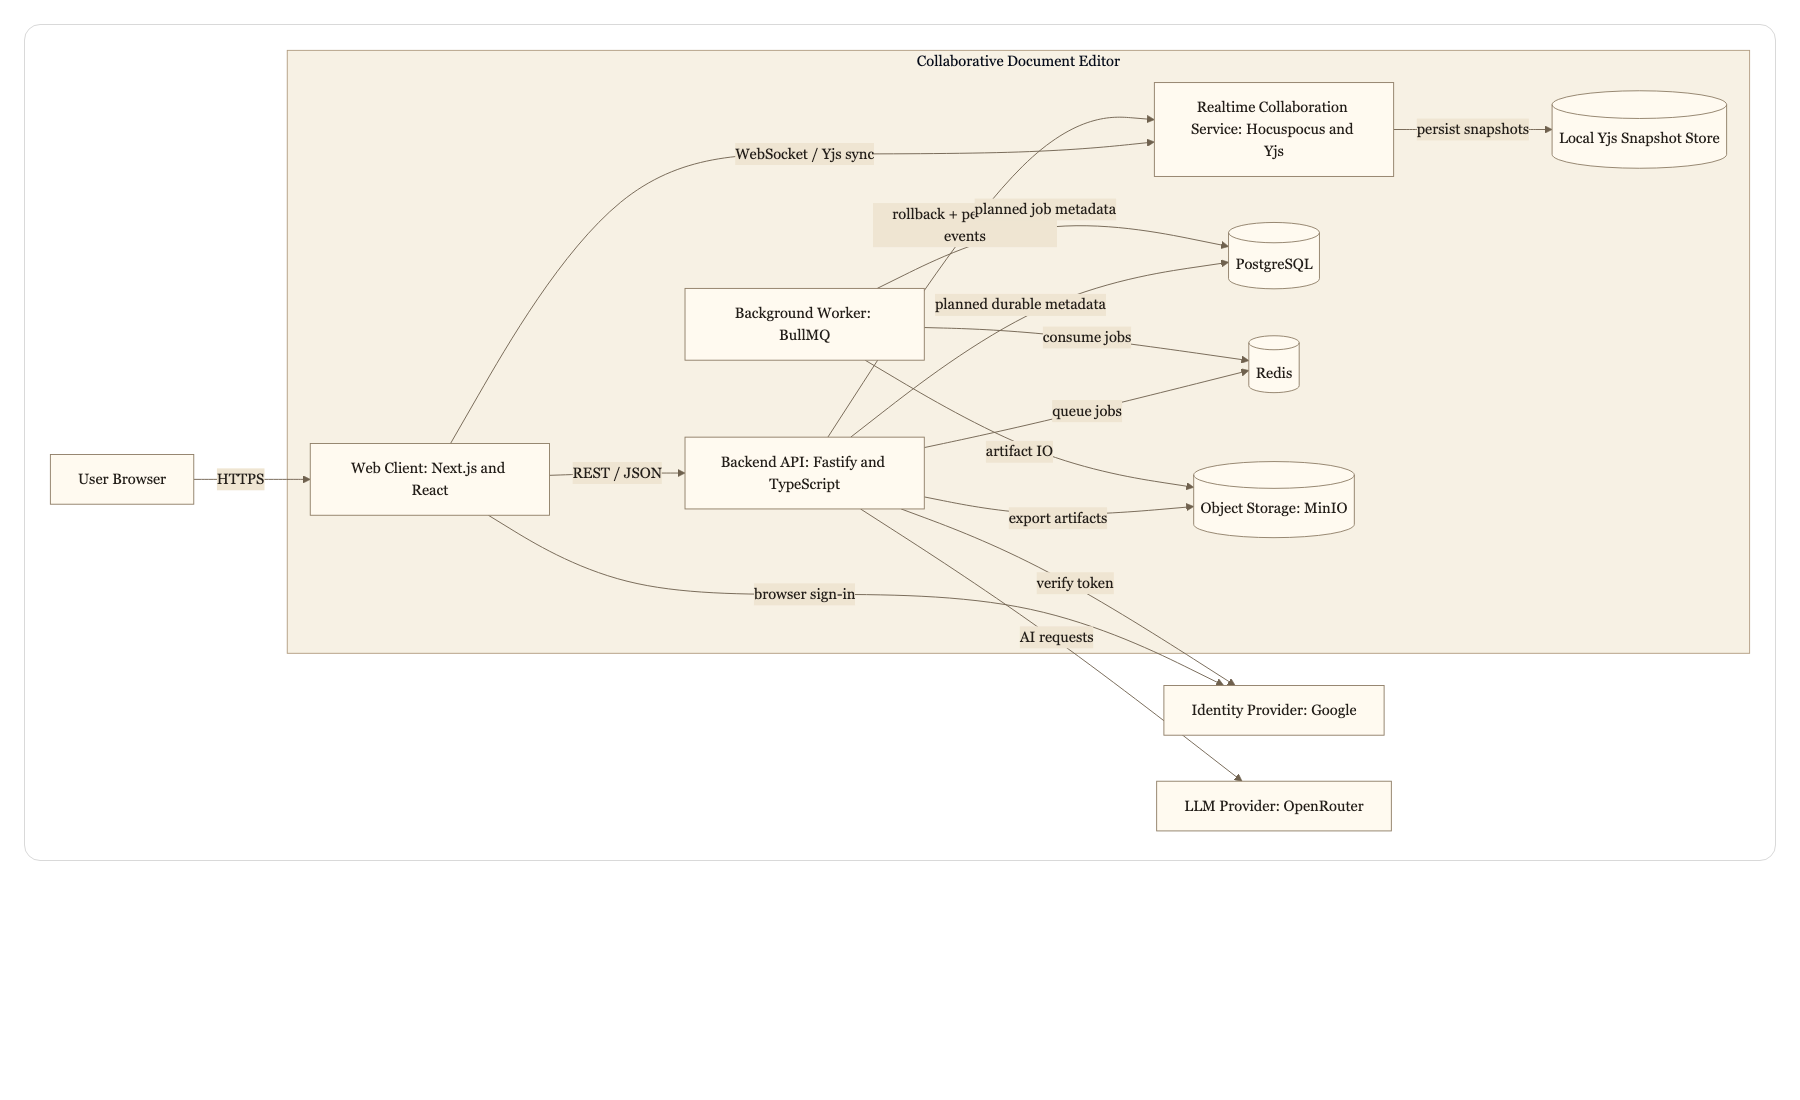
\includegraphics[width=\textwidth,height=0.42\textheight,keepaspectratio]{docs/diagrams/generated/ai1220-container-view.png}
\end{figure}

\paragraph{Container responsibilities}\label{container-responsibilities}

\begin{table}[h]
\small
\begin{tabularx}{\textwidth}{@{}L{40mm}Y L{34mm}@{}}
\toprule
Container & Responsibility & Technology choice \\
\midrule
Web Client & Editor UI, document list, comments panel, AI actions, auth handoff, local draft recovery & Next.js, React, TypeScript \\
Backend API & Document CRUD, comments, sharing, versions, exports, AI orchestration, session bootstrap & Fastify, Node.js, TypeScript \\
Realtime Collaboration Service & Live editing sync, presence, reconnect behavior, writer slots, stateless collab events & Hocuspocus, Yjs, WebSocket \\
Background Worker & Async job execution for exports and future durable AI or revision work & BullMQ worker \\
PostgreSQL & Provisioned relational store for durable metadata & PostgreSQL \\
Redis & Queue coordination and transient worker state & Redis \\
Object Storage & Export artifacts and future retained snapshots & MinIO / S3-compatible storage \\
Local Yjs Snapshot Store & Current persisted realtime document content & Filesystem-backed \texttt{.bin} snapshots \\
\bottomrule
\end{tabularx}
\end{table}

\subsubsection{3.3 Level 3: Component Diagram for AI Service
Path}\label{33-level-3-component-diagram-for-ai-service-path}

The current repository does not run AI as a separate deployable service.
Instead, the AI workflow is implemented as an API-side module with a
provider adapter. The component-level design below reflects the actual
code path.

Mermaid source:
\href{/Users/rayan.banerjee/courses/software\%20project/docs/diagrams/ai1220-ai-component-view.mmd}{ai1220-ai-component-view.mmd}

\begin{figure}[h]
\centering
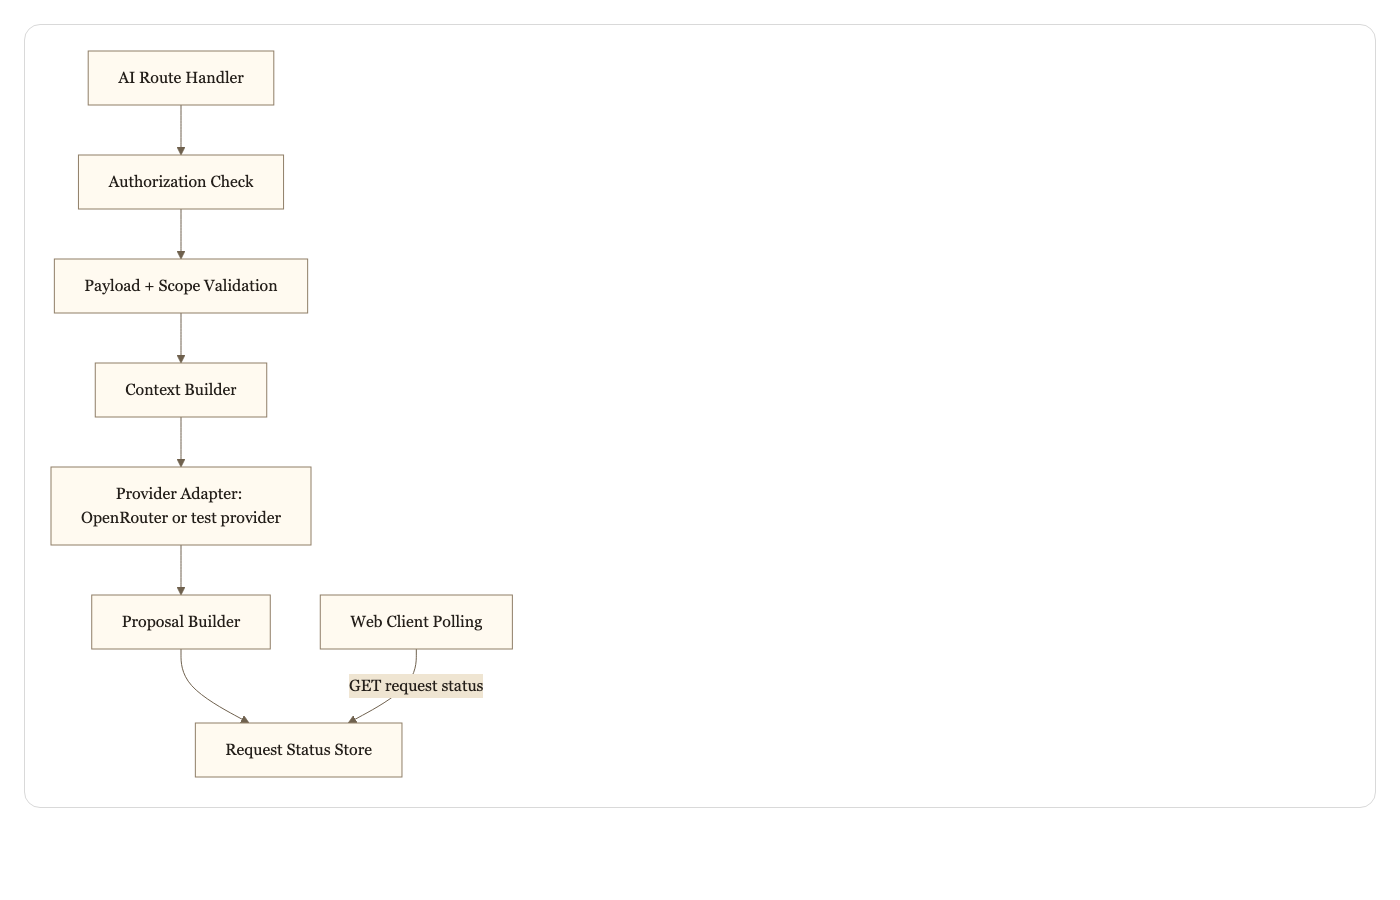
\includegraphics[width=\textwidth,height=0.3\textheight,keepaspectratio]{docs/diagrams/generated/ai1220-ai-component-view.png}
\end{figure}

The AI path:

\begin{itemize}
\tightlist
\item
  validates that the user has permission to invoke AI for the document
\item
  validates operation type and scope
\item
  constructs request context from the selected text and surrounding
  content
\item
  calls the provider adapter
\item
  stores request/proposal state
\item
  returns a proposal that the user must explicitly accept or reject
\end{itemize}

\subsection{4. Feature Decomposition}\label{4-feature-decomposition}

\begin{table}[h]
\small
\begin{tabularx}{\textwidth}{@{}L{31mm}Y L{33mm} L{31mm}@{}}
\toprule
Module & What it does & Depends on & Exposes \\
\midrule
Editor frontend & Rich-text editing UI, selection, comments, AI actions, version UI & API, realtime collaboration service & User interactions and editor commands \\
Frontend state layer & Auth state, document state, comment state, reconnect status & Editor frontend, API & State selectors and actions \\
Realtime sync layer & Yjs updates, presence, reconnect, writer slots & Collaboration service & Session join, sync, presence updates \\
API layer & Documents, comments, sharing, versions, exports, AI requests & Auth, storage, worker, realtime service & REST endpoints \\
AI integration path & Proposal generation and lifecycle tracking & API, provider adapter & Request and status interfaces \\
Auth module & Sign-in, session validation, role checks & Identity provider, API & Session cookie and auth context \\
Storage/versioning module & Metadata and revision management & Postgres, object storage, local snapshots & Revision list, restore, export refs \\
\bottomrule
\end{tabularx}
\end{table}

This decomposition keeps frontend interaction, REST business logic,
realtime sync, and AI orchestration separated enough for team delivery
and testing.

\subsection{5. AI Integration Design}\label{5-ai-integration-design}

\subsubsection{5.1 Context and Scope}\label{51-context-and-scope}

The default AI context is the selected text plus limited surrounding
context for coherence. Full-document scope should be reserved for
summarization or structural operations because it costs more and
increases latency.

Trade-offs:

\begin{itemize}
\tightlist
\item
  selection-only scope is faster and cheaper
\item
  full-document scope is more accurate for global operations
\item
  long documents should be constrained by operation-specific context
  rules
\end{itemize}

\subsubsection{5.2 Suggestion UX}\label{52-suggestion-ux}

AI output is presented as a proposal in the right utility panel rather
than directly editing the document.

\begin{itemize}
\tightlist
\item
  users can accept or reject proposals
\item
  accepted changes remain part of the normal editor history
\item
  proposals are linked to the original selection and request type
\item
  AI actions are triggered from the editor context menu
\item
  the UI polls request status until a proposal is ready
\end{itemize}

\subsubsection{5.3 AI During
Collaboration}\label{53-ai-during-collaboration}

The selected region is not locked while AI is running.

\begin{itemize}
\tightlist
\item
  the requester sees a pending or generating state
\item
  other collaborators can continue editing
\item
  if the source region changes, the proposal may become stale
\item
  stale detection is tracked in the AI request lifecycle
\end{itemize}

\subsubsection{5.4 Prompt Design}\label{54-prompt-design}

Prompt logic should remain template-based rather than being scattered
across route handlers.

\begin{itemize}
\tightlist
\item
  operation-specific templates should exist for rewrite, summarize,
  translate, and restructure
\item
  templates should accept structured input such as selected text, scope,
  and optional prompt
\item
  prompt logic should remain isolated from HTTP transport logic
\end{itemize}

\subsubsection{5.5 Model and Cost
Strategy}\label{55-model-and-cost-strategy}

Different models may be used for different tasks.

\begin{itemize}
\tightlist
\item
  lighter models can serve rewrite and formatting
\item
  stronger models can serve summarize and restructure
\item
  cost/latency controls should eventually include quotas or per-team
  limits
\item
  when no real key is configured, normal runtime should fail honestly
  rather than silently mock
\end{itemize}

\subsection{6. API Design}\label{6-api-design}

\subsubsection{6.1 API Style}\label{61-api-style}

\begin{itemize}
\tightlist
\item
  REST is used for document CRUD, sharing, versions, exports, comments,
  and AI request submission
\item
  a realtime push channel is used for collaborative editing and presence
\item
  asynchronous job patterns are used for worker-oriented flows
\end{itemize}

This split keeps business operations explicit while preserving
low-latency collaboration.

\subsubsection{6.2 Core API Contract}\label{62-core-api-contract}

\paragraph{Document CRUD}\label{document-crud}

\begin{table}[h]
\small
\begin{tabularx}{\textwidth}{@{}L{14mm}L{44mm}Y@{}}
\toprule
Method & Endpoint & Purpose \\
\midrule
POST & \texttt{/v1/documents} & Create document \\
GET & \texttt{/v1/documents} & List visible documents \\
GET & \texttt{/v1/documents/\{id\}} & Load metadata and permissions \\
PATCH & \texttt{/v1/documents/\{id\}} & Rename document \\
DELETE & \texttt{/v1/documents/\{id\}} & Archive document \\
\bottomrule
\end{tabularx}
\end{table}

Example response:

\begin{Shaded}
\begin{Highlighting}[]
\FunctionTok{\{}
  \DataTypeTok{"document"}\FunctionTok{:} \FunctionTok{\{}
    \DataTypeTok{"id"}\FunctionTok{:} \StringTok{"doc\_123"}\FunctionTok{,}
    \DataTypeTok{"title"}\FunctionTok{:} \StringTok{"Design Notes"}\FunctionTok{,}
    \DataTypeTok{"createdAt"}\FunctionTok{:} \StringTok{"2026{-}04{-}03T00:00:00.000Z"}\FunctionTok{,}
    \DataTypeTok{"updatedAt"}\FunctionTok{:} \StringTok{"2026{-}04{-}03T00:00:00.000Z"}\FunctionTok{,}
    \DataTypeTok{"archivedAt"}\FunctionTok{:} \KeywordTok{null}\FunctionTok{,}
    \DataTypeTok{"permissions"}\FunctionTok{:} \FunctionTok{\{}
      \DataTypeTok{"role"}\FunctionTok{:} \StringTok{"owner"}\FunctionTok{,}
      \DataTypeTok{"canView"}\FunctionTok{:} \KeywordTok{true}\FunctionTok{,}
      \DataTypeTok{"canComment"}\FunctionTok{:} \KeywordTok{true}\FunctionTok{,}
      \DataTypeTok{"canEdit"}\FunctionTok{:} \KeywordTok{true}\FunctionTok{,}
      \DataTypeTok{"canShare"}\FunctionTok{:} \KeywordTok{true}\FunctionTok{,}
      \DataTypeTok{"canExport"}\FunctionTok{:} \KeywordTok{true}\FunctionTok{,}
      \DataTypeTok{"canUseAi"}\FunctionTok{:} \KeywordTok{true}\FunctionTok{,}
      \DataTypeTok{"canRollback"}\FunctionTok{:} \KeywordTok{true}
    \FunctionTok{\}}
  \FunctionTok{\}}
\FunctionTok{\}}
\end{Highlighting}
\end{Shaded}

\paragraph{Realtime session
management}\label{realtime-session-management}

\begin{table}[h]
\small
\begin{tabularx}{\textwidth}{@{}L{14mm}L{54mm}Y@{}}
\toprule
Method & Endpoint & Purpose \\
\midrule
POST & \texttt{/v1/documents/\{id\}/sessions} & Join an editing session and receive realtime credentials \\
\bottomrule
\end{tabularx}
\end{table}

Example response:

\begin{Shaded}
\begin{Highlighting}[]
\FunctionTok{\{}
  \DataTypeTok{"session"}\FunctionTok{:} \FunctionTok{\{}
    \DataTypeTok{"documentId"}\FunctionTok{:} \StringTok{"doc\_123"}\FunctionTok{,}
    \DataTypeTok{"joinedAt"}\FunctionTok{:} \StringTok{"2026{-}04{-}03T00:00:00.000Z"}\FunctionTok{,}
    \DataTypeTok{"resumedFromSessionId"}\FunctionTok{:} \KeywordTok{null}\FunctionTok{,}
    \DataTypeTok{"self"}\FunctionTok{:} \FunctionTok{\{}
      \DataTypeTok{"sessionId"}\FunctionTok{:} \StringTok{"sess\_789"}\FunctionTok{,}
      \DataTypeTok{"documentId"}\FunctionTok{:} \StringTok{"doc\_123"}\FunctionTok{,}
      \DataTypeTok{"userId"}\FunctionTok{:} \StringTok{"google:user\_owner"}\FunctionTok{,}
      \DataTypeTok{"displayName"}\FunctionTok{:} \StringTok{"Owner Demo"}\FunctionTok{,}
      \DataTypeTok{"role"}\FunctionTok{:} \StringTok{"owner"}\FunctionTok{,}
      \DataTypeTok{"accessLevel"}\FunctionTok{:} \StringTok{"write"}\FunctionTok{,}
      \DataTypeTok{"isPresent"}\FunctionTok{:} \KeywordTok{true}\FunctionTok{,}
      \DataTypeTok{"lastSeenAt"}\FunctionTok{:} \StringTok{"2026{-}04{-}03T00:00:00.000Z"}\FunctionTok{,}
      \DataTypeTok{"connectionStatus"}\FunctionTok{:} \StringTok{"active"}
    \FunctionTok{\},}
    \DataTypeTok{"collaborators"}\FunctionTok{:} \OtherTok{[]}
  \FunctionTok{\},}
  \DataTypeTok{"websocketUrl"}\FunctionTok{:} \StringTok{"ws://localhost:4001?documentName=doc\_123\&token=..."}\FunctionTok{,}
  \DataTypeTok{"token"}\FunctionTok{:} \StringTok{"signed{-}session{-}token"}
\FunctionTok{\}}
\end{Highlighting}
\end{Shaded}

\paragraph{AI assistant invocation}\label{ai-assistant-invocation}

\begin{table}[h]
\small
\begin{tabularx}{\textwidth}{@{}L{14mm}L{72mm}Y@{}}
\toprule
Method & Endpoint & Purpose \\
\midrule
POST & \texttt{/v1/documents/\{id\}/ai/requests} & Submit AI operation \\
GET & \texttt{/v1/documents/\{id\}/ai/requests/\{requestId\}} & Poll request status \\
POST & \texttt{/v1/documents/\{id\}/ai/proposals/accept} & Accept proposal \\
POST & \texttt{/v1/documents/\{id\}/ai/proposals/reject} & Reject proposal \\
\bottomrule
\end{tabularx}
\end{table}

Example request:

\begin{Shaded}
\begin{Highlighting}[]
\FunctionTok{\{}
  \DataTypeTok{"action"}\FunctionTok{:} \StringTok{"summarize"}\FunctionTok{,}
  \DataTypeTok{"prompt"}\FunctionTok{:} \KeywordTok{null}\FunctionTok{,}
  \DataTypeTok{"context"}\FunctionTok{:} \FunctionTok{\{}
    \DataTypeTok{"scope"}\FunctionTok{:} \StringTok{"selection"}\FunctionTok{,}
    \DataTypeTok{"selectedText"}\FunctionTok{:} \StringTok{"some selected content"}\FunctionTok{,}
    \DataTypeTok{"surroundingText"}\FunctionTok{:} \KeywordTok{null}
  \FunctionTok{\},}
  \DataTypeTok{"maskPersonalData"}\FunctionTok{:} \KeywordTok{false}
\FunctionTok{\}}
\end{Highlighting}
\end{Shaded}

Example status response:

\begin{Shaded}
\begin{Highlighting}[]
\FunctionTok{\{}
  \DataTypeTok{"requestId"}\FunctionTok{:} \StringTok{"air\_456"}\FunctionTok{,}
  \DataTypeTok{"status"}\FunctionTok{:} \StringTok{"running"}\FunctionTok{,}
  \DataTypeTok{"startedAt"}\FunctionTok{:} \StringTok{"2026{-}04{-}03T00:00:00.000Z"}\FunctionTok{,}
  \DataTypeTok{"completedAt"}\FunctionTok{:} \KeywordTok{null}\FunctionTok{,}
  \DataTypeTok{"errorMessage"}\FunctionTok{:} \KeywordTok{null}\FunctionTok{,}
  \DataTypeTok{"proposal"}\FunctionTok{:} \KeywordTok{null}
\FunctionTok{\}}
\end{Highlighting}
\end{Shaded}

\paragraph{Comments}\label{comments}

\begin{table}[h]
\small
\begin{tabularx}{\textwidth}{@{}L{14mm}L{46mm}Y@{}}
\toprule
Method & Endpoint & Purpose \\
\midrule
GET & \texttt{/v1/documents/\{id\}/comments} & List comments \\
POST & \texttt{/v1/documents/\{id\}/comments} & Create comment \\
\bottomrule
\end{tabularx}
\end{table}

\paragraph{Sharing and permissions}\label{sharing-and-permissions}

\begin{table}[h]
\small
\begin{tabularx}{\textwidth}{@{}L{14mm}L{68mm}Y@{}}
\toprule
Method & Endpoint & Purpose \\
\midrule
POST & \texttt{/v1/documents/\{id\}/invitations} & Create invitation \\
POST & \texttt{/v1/invitations/accept} & Accept invitation \\
PATCH & \texttt{/v1/documents/\{id\}/members/\{userId\}} & Update member role \\
DELETE & \texttt{/v1/documents/\{id\}/members/\{userId\}} & Revoke access \\
\bottomrule
\end{tabularx}
\end{table}

\subsubsection{6.3 Long-Running AI
Operations}\label{63-long-running-ai-operations}

The client submits an AI request and then polls status until the request
reaches a terminal state.

Possible status values include:

\begin{itemize}
\tightlist
\item
  \texttt{queued}
\item
  \texttt{running}
\item
  \texttt{succeeded}
\item
  \texttt{failed}
\item
  \texttt{cancelled}
\item
  \texttt{stale}
\end{itemize}

\subsubsection{6.4 Error Handling}\label{64-error-handling}

Clients should distinguish common failure cases using the standard API
error envelope.

\begin{table}[h]
\small
\begin{tabularx}{\textwidth}{@{}L{38mm}Y@{}}
\toprule
Case & API signal \\
\midrule
AI still running & \texttt{200} with status \texttt{queued} or \texttt{running} \\
AI failed & \texttt{200} status payload with \texttt{failed}, or route-level provider/config error \\
Forbidden action & \texttt{403} \\
Document not found & \texttt{404} \\
Auth required & \texttt{401} \\
\bottomrule
\end{tabularx}
\end{table}

\subsection{7. Authentication and
Authorization}\label{7-authentication-and-authorization}

Authentication identifies users, links actions to accounts, and enforces
sharing rules.

Expected user types:

\begin{itemize}
\tightlist
\item
  document owners
\item
  editors
\item
  commenters
\item
  viewers
\end{itemize}

\subsubsection{Roles and capabilities}\label{roles-and-capabilities}

\begin{table}[h]
\small
\begin{tabularx}{\textwidth}{@{}L{22mm}Y@{}}
\toprule
Role & Capabilities \\
\midrule
Owner & Full control, including sharing, export, version restore, commenting, editing, and AI access \\
Editor & Read, edit, comment, invoke AI, view versions, and export \\
Commenter & Read and comment only \\
Viewer & Read only \\
\bottomrule
\end{tabularx}
\end{table}

\subsubsection{Current implementation
notes}\label{current-implementation-notes}

\begin{itemize}
\tightlist
\item
  sign-in uses Google Identity Services in the browser
\item
  the API validates Google ID tokens and issues signed session cookies
\item
  the collab service authenticates realtime sessions using the signed
  token issued by the API
\item
  local development currently auto-grants cross-account document access
  to simplify collaboration testing
\end{itemize}

Privacy considerations for third-party AI:

\begin{itemize}
\tightlist
\item
  selected content may leave the primary system boundary when sent to
  the LLM provider
\item
  the minimum viable context should be sent
\item
  request logs should avoid retaining unnecessary sensitive content
\end{itemize}

\subsection{8. Communication Model}\label{8-communication-model}

The system uses push-based realtime communication for editing sessions
and standard request-response APIs for business operations.

\subsubsection{8.1 Opening a Shared
Document}\label{81-opening-a-shared-document}

Mermaid source:
\href{/Users/rayan.banerjee/courses/software\%20project/docs/diagrams/ai1220-open-shared-document-sequence.mmd}{ai1220-open-shared-document-sequence.mmd}

\begin{figure}[h]
\centering
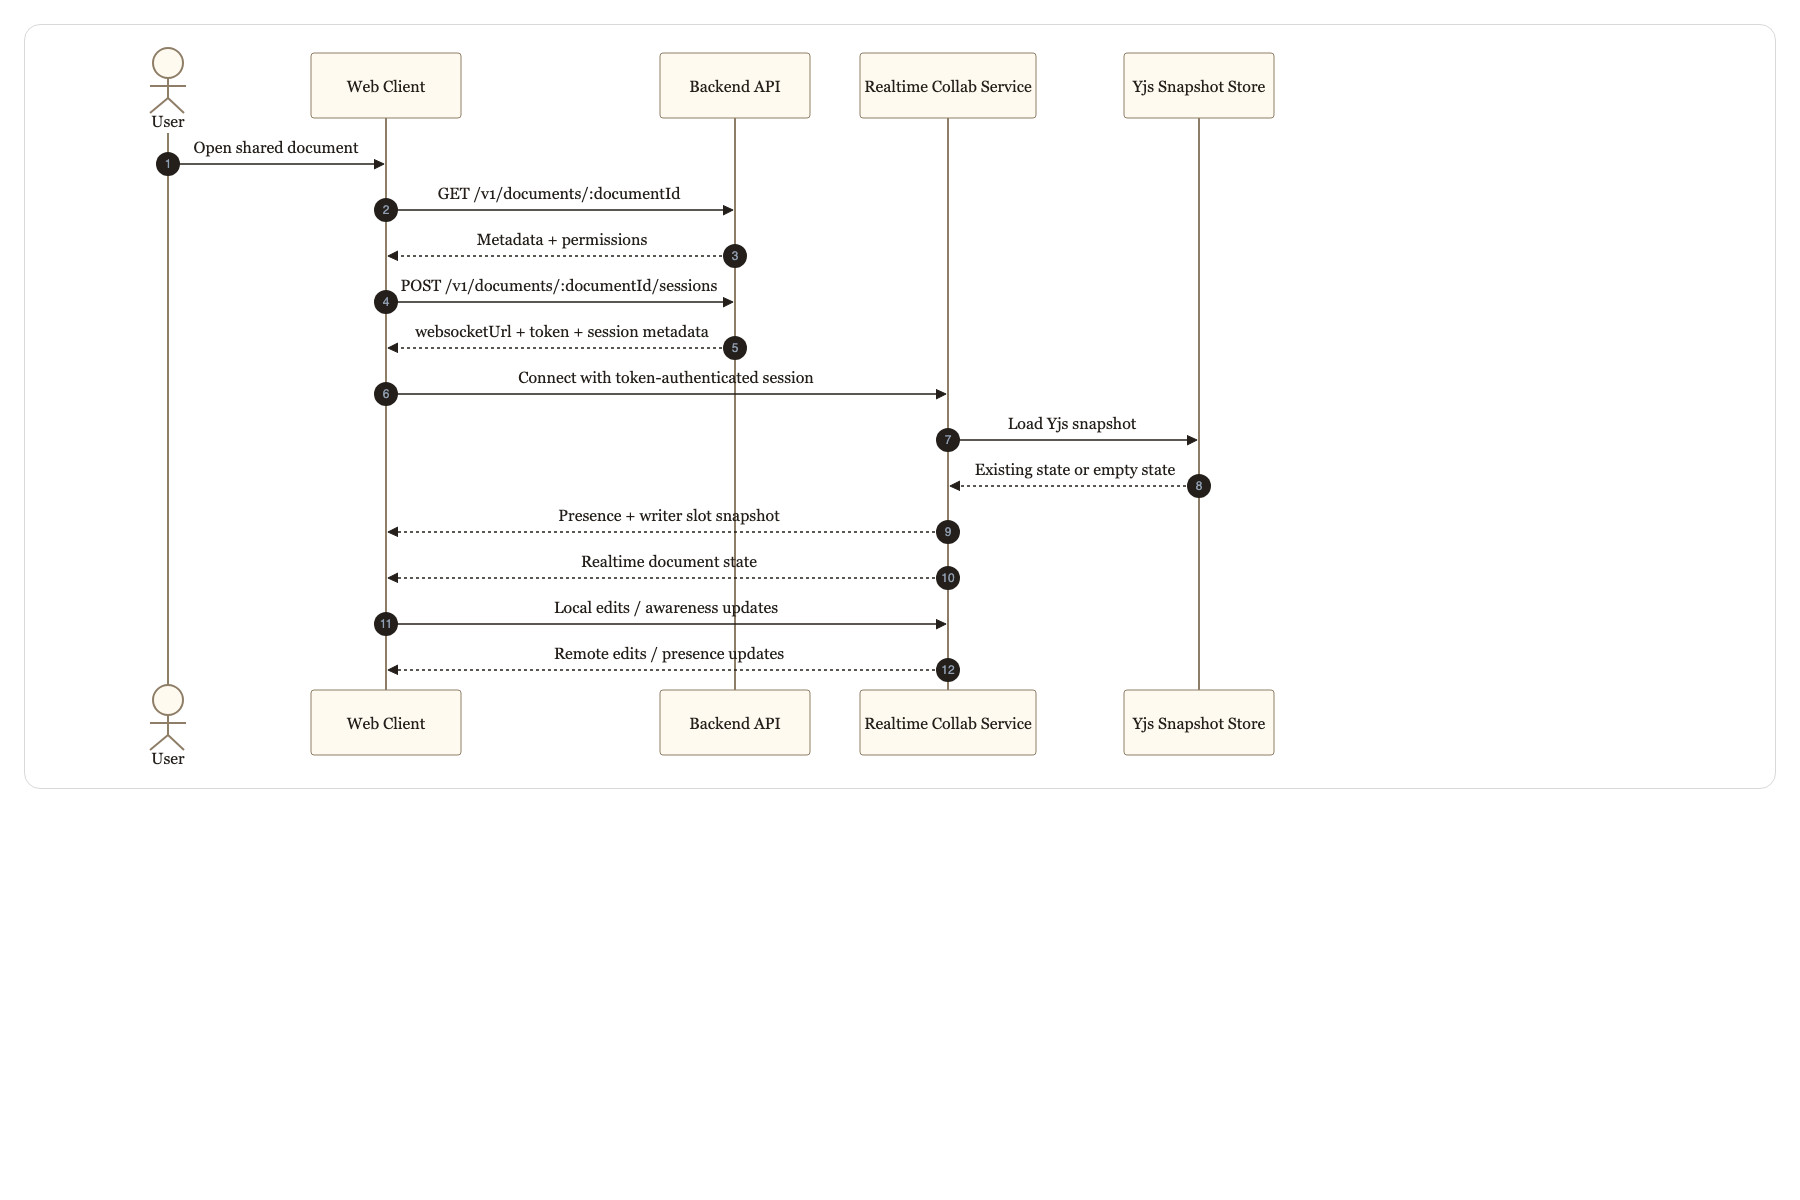
\includegraphics[width=\textwidth,height=0.42\textheight,keepaspectratio]{docs/diagrams/generated/ai1220-open-shared-document-sequence.png}
\end{figure}

\subsubsection{8.2 Connectivity Loss and
Recovery}\label{82-connectivity-loss-and-recovery}

If a user disconnects:

\begin{itemize}
\tightlist
\item
  local unsent edits are buffered in the browser
\item
  the UI shows offline or reconnecting state
\item
  when connectivity returns, the client rejoins the session
\item
  the collab service reloads persisted Yjs state and resumes
  synchronization
\end{itemize}

\subsubsection{8.3 Presence and Cursor
Behavior}\label{83-presence-and-cursor-behavior}

\begin{itemize}
\tightlist
\item
  connected collaborators can see presence updates in near real time
\item
  writer slots distinguish active writers from queued or read-only
  sessions
\item
  viewer sessions are represented in presence summaries but do not gain
  write capability
\item
  presence entries are deduplicated by user to avoid duplicated viewer
  rows across reconnects
\end{itemize}

\subsection{9. Code Structure and Repository
Organization}\label{9-code-structure-and-repository-organization}

\subsubsection{9.1 Monorepo vs
Multi-repo}\label{91-monorepo-vs-multi-repo}

A monorepo is the better fit for this project because frontend, backend,
collab, worker, and shared contracts evolve together.

\subsubsection{9.2 Current Repository
Tree}\label{92-current-repository-tree}

\begin{verbatim}
repo/
|-- apps/
|   |-- web/
|   |-- api/
|   |-- collab/
|   `-- worker/
|-- packages/
|   |-- authz/
|   |-- editor-schema/
|   |-- shared-types/
|   |-- test-fixtures/
|   `-- ui/
|-- docs/
|   |-- adr/
|   |-- api/
|   |-- diagrams/
|   |-- process/
|   |-- specs/
|   `-- tasks/
|-- infrastructure/
|   |-- docker/
|   `-- scripts/
|-- tests/
`-- README.md
\end{verbatim}

\subsubsection{9.3 Shared Code}\label{93-shared-code}

Shared contracts and editor definitions live in workspace packages so
both frontend and backend can import them without duplicating
request/response logic.

\subsubsection{9.4 Configuration
Management}\label{94-configuration-management}

\begin{itemize}
\tightlist
\item
  secrets live in app-specific \texttt{.env.local} files
\item
  \texttt{.env.example} files remain templates only
\item
  Google/OpenRouter credentials should not be committed
\end{itemize}

\subsubsection{9.5 Testing Structure}\label{95-testing-structure}

\begin{itemize}
\tightlist
\item
  API unit/integration tests live under \texttt{apps/api/tests}
\item
  collab tests live under \texttt{apps/collab/tests}
\item
  web tests live under \texttt{apps/web/tests}
\item
  root tests validate cross-repo foundation behavior
\end{itemize}

\subsection{10. Data Model}\label{10-data-model}

\subsubsection{10.1 Storage Approach}\label{101-storage-approach}

Current persistence is hybrid:

\begin{itemize}
\tightlist
\item
  document metadata: API in-memory store
\item
  comments: API in-memory store
\item
  realtime document content: persisted Yjs snapshots on local disk
\item
  queue coordination: Redis
\item
  relational storage: Postgres provisioned but not yet the primary store
  for all runtime entities
\end{itemize}

Each document requires more than raw content:

\begin{itemize}
\tightlist
\item
  title
\item
  owner and memberships
\item
  timestamps
\item
  archived status
\item
  current collaborative state
\item
  version and AI proposal references
\end{itemize}

\subsubsection{10.2 Entity Relationship
Diagram}\label{102-entity-relationship-diagram}

Mermaid source:
\href{/Users/rayan.banerjee/courses/software\%20project/docs/diagrams/ai1220-entity-relationship.mmd}{ai1220-entity-relationship.mmd}

\begin{figure}[h]
\centering
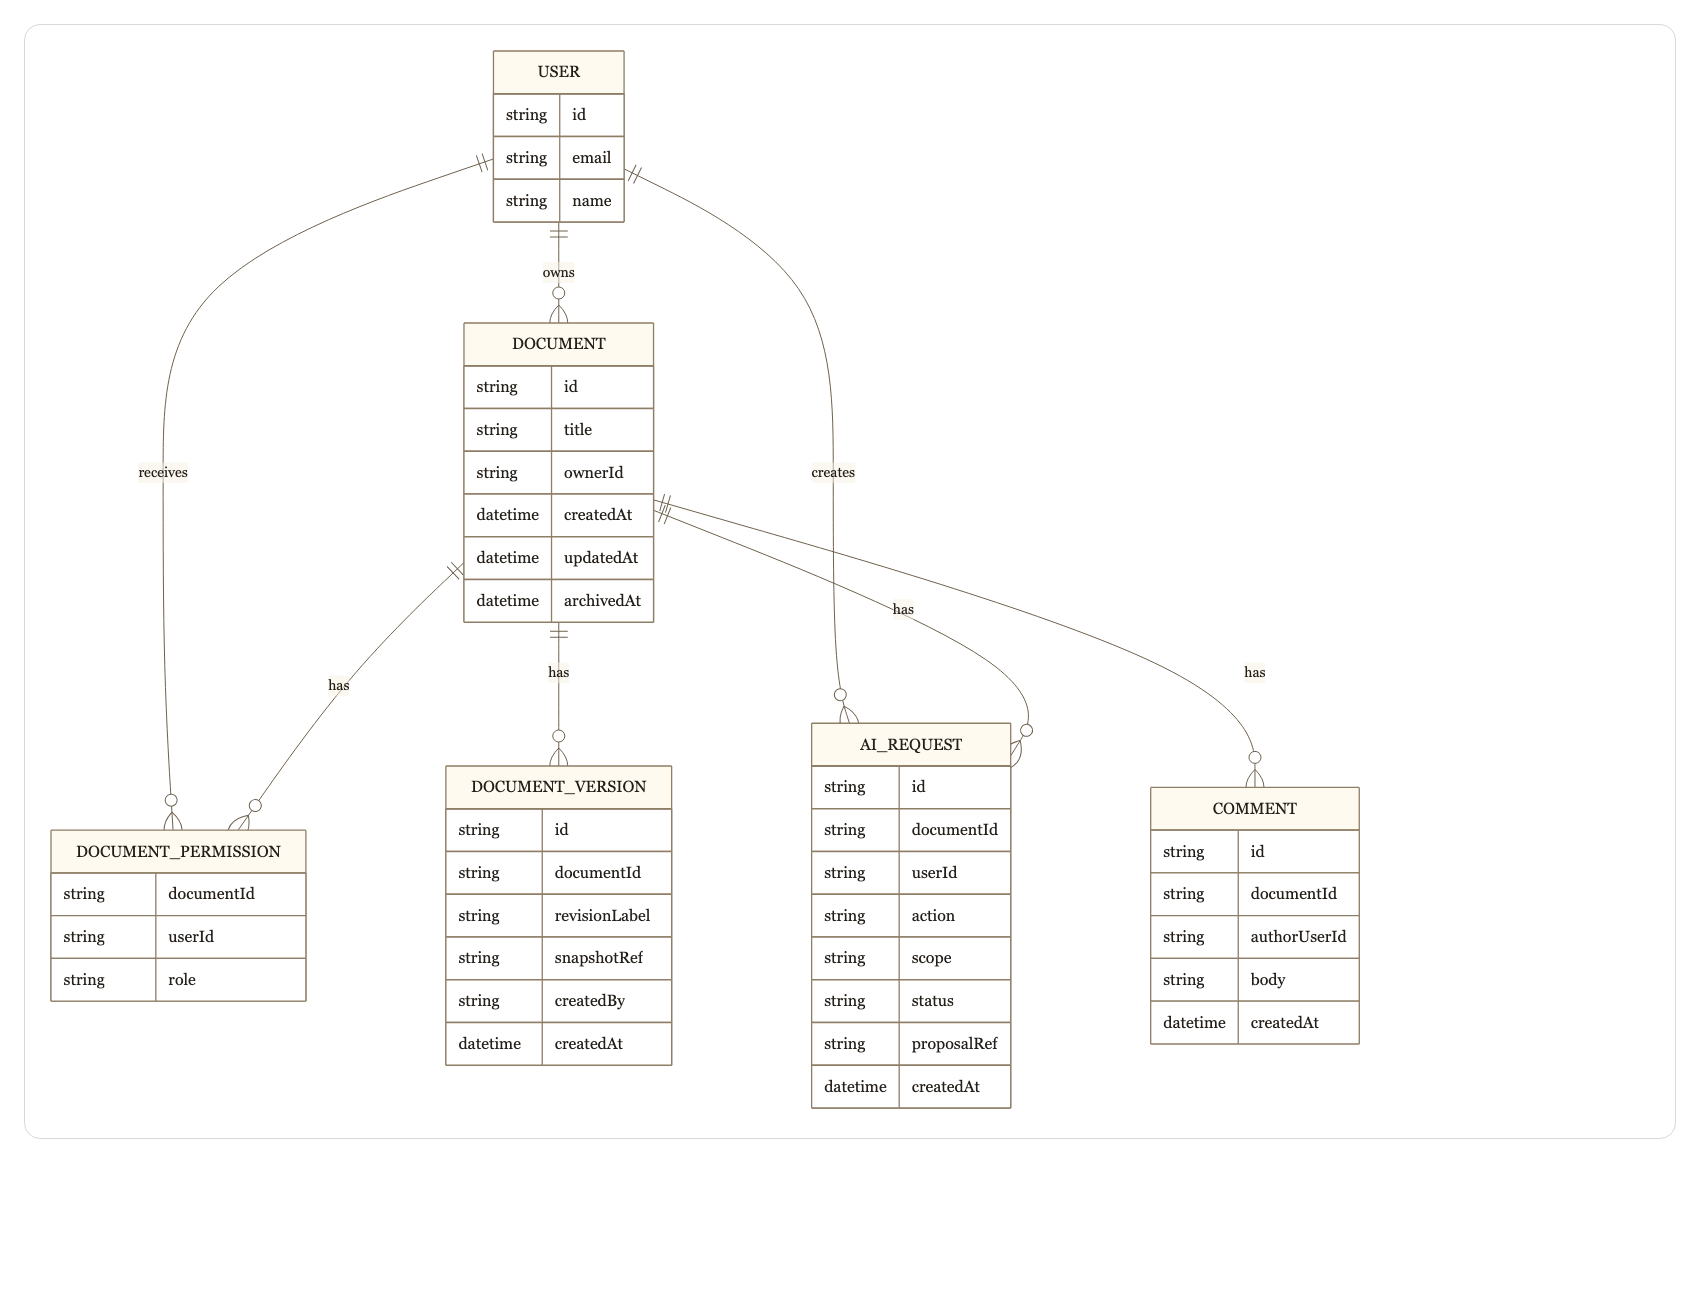
\includegraphics[width=\textwidth,height=0.42\textheight,keepaspectratio]{docs/diagrams/generated/ai1220-entity-relationship.png}
\end{figure}

\subsubsection{10.3 Versioning, Permissions, and AI
History}\label{103-versioning-permissions-and-ai-history}

\begin{itemize}
\tightlist
\item
  version history allows owners and editors to inspect and restore prior
  document states
\item
  permissions are modeled separately so documents can be shared across
  multiple users
\item
  AI requests record operation type, scope, status, and proposal
  lifecycle
\end{itemize}

\subsection{11. Architecture Decision
Records}\label{11-architecture-decision-records}

The repository already contains a broader ADR set under
\href{/Users/rayan.banerjee/courses/software\%20project/docs/adr}{docs/adr}.
For the assignment, the four core ADRs are summarized here in the
expected format.

\subsubsection{ADR-1: Use a CRDT-based collaboration
model}\label{adr-1-use-a-crdt-based-collaboration-model}

Status: Accepted

Context: Multiple users need to edit the same document concurrently,
including after temporary disconnects.

Decision: Use a Yjs/Hocuspocus-based realtime synchronization service
with persisted Yjs snapshots.

Consequences:

\begin{itemize}
\tightlist
\item
  strong support for concurrent editing and reconnect behavior
\item
  higher implementation complexity than a save-based editor
\end{itemize}

Alternatives considered:

\begin{itemize}
\tightlist
\item
  document locking, rejected because it harms collaboration
\item
  last-write-wins, rejected because it risks silent data loss
\end{itemize}

\subsubsection{ADR-2: AI returns proposals, not direct
edits}\label{adr-2-ai-returns-proposals-not-direct-edits}

Status: Accepted

Context: AI responses can arrive after the underlying document selection
has changed.

Decision: AI responses are shown as reviewable proposals that users
explicitly accept or reject.

Consequences:

\begin{itemize}
\tightlist
\item
  safer collaboration and clearer user control
\item
  extra UI work for proposal review
\end{itemize}

Alternatives considered:

\begin{itemize}
\tightlist
\item
  direct inline replacement, rejected because it can overwrite newer
  edits
\end{itemize}

\subsubsection{ADR-3: Use REST for business APIs and push-based sync for
collaboration}\label{adr-3-use-rest-for-business-apis-and-push-based-sync-for-collaboration}

Status: Accepted

Context: CRUD operations and realtime editing have different
communication needs.

Decision: Use REST for standard business operations and a persistent
realtime channel for collaborative editing.

Consequences:

\begin{itemize}
\tightlist
\item
  clear API boundaries
\item
  two communication patterns instead of one
\end{itemize}

Alternatives considered:

\begin{itemize}
\tightlist
\item
  all polling, rejected because it harms collaboration UX
\item
  all traffic through one custom socket protocol, rejected because it
  complicates standard API work
\end{itemize}

\subsubsection{ADR-4: Use a monorepo with shared
contracts}\label{adr-4-use-a-monorepo-with-shared-contracts}

Status: Accepted

Context: Frontend, backend, worker, and collab contracts evolve
together.

Decision: Keep project code in one repository with shared packages for
types, auth rules, UI primitives, and editor schema.

Consequences:

\begin{itemize}
\tightlist
\item
  simpler coordination for a student team
\item
  requires discipline to keep module boundaries clean
\end{itemize}

Alternatives considered:

\begin{itemize}
\tightlist
\item
  separate repositories, rejected because it adds overhead too early
\end{itemize}

\subsection{12. Conclusion}\label{12-conclusion}

This architecture is no longer just a conceptual target. The current
repository already implements the main structural choices: a monorepo,
REST business APIs, a dedicated realtime collaboration service,
proposal-based AI, and shared contract packages. The main remaining work
is to replace prototype persistence and local-development shortcuts with
durable production-grade storage and deployment behavior.

\end{document}
